
\section{Seismic Catalog}


\begin{figure*}[t] 
	\centering
	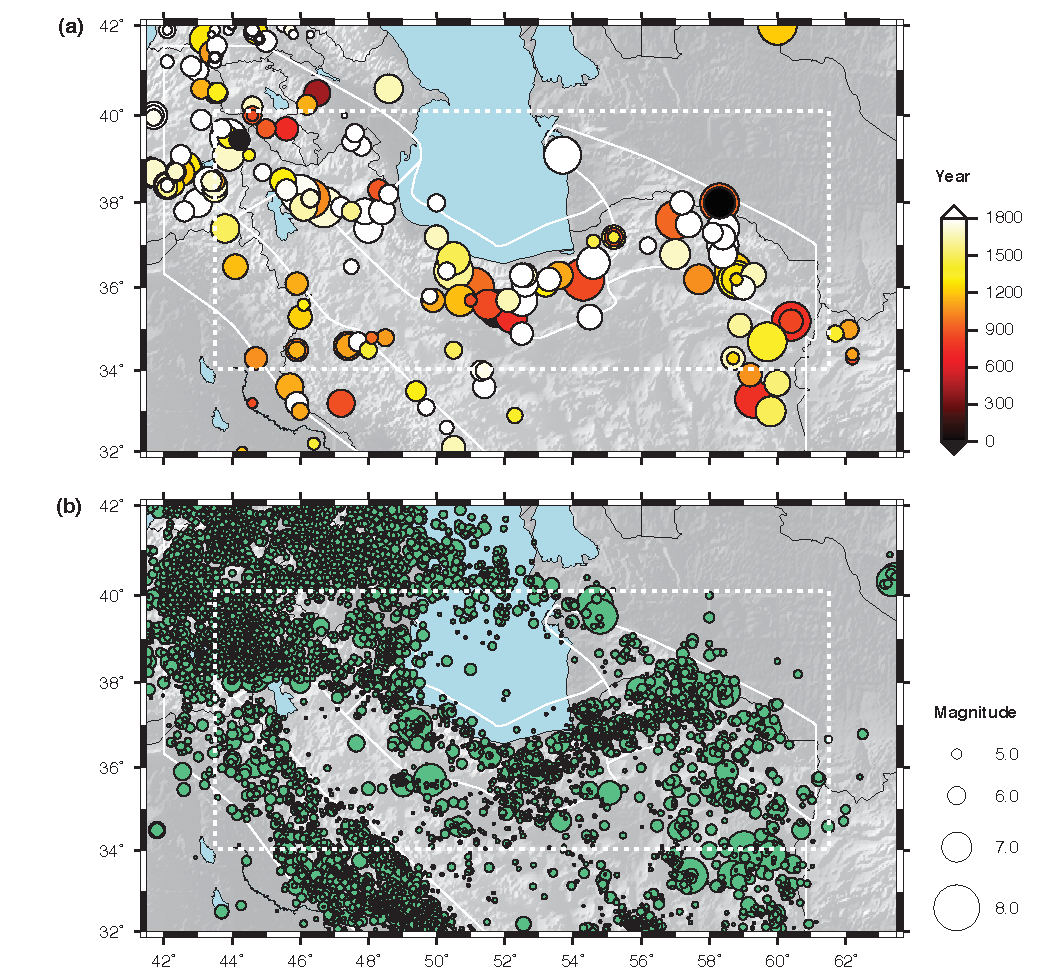
\includegraphics[width=0.9\textwidth]{figures/pdf/figure-03}
	\caption{Location of events considered in the compiled seismic catalog. (a) Historical seismicity prior to 1900 for $M_w \geq 4$ \citep[after][]{Zare2014}. (b) Instrumental seismicity up until December 2015 for $M_w \geq 3$ (IIEES) and $M_w \geq 4$ \citep[after][]{Zare2014}. Size of symbols is proportional to the magnitude of the events. In the case of the historical seismicity catalog, the color fill indicates the year of the event. The borderlines of the seismic zones shown in Fig.~\ref{fig:iran} are shown in the background in white, along with the light gray shaded relief.}
	\label{fig:catalog}
\end{figure*}

\subsection{Composition}

A fundamental step in regional seismic hazard analysis is the composition of a reliable seismic catalog that includes both historically documented and instrumentally recorded earthquakes. Nowadays, instrumental datasets are easily accessible through international, regional, and local agencies. Historical data, on the other hand, lends itself to subjective interpretation. Notable previous efforts to compose uniform earthquake catalogs for Iran include but are not limited to \citet{Ambraseys_1982_Book}, \citet{moinfar1994}, and \citet{Berberian_1995_Tech}. These studies, however, differ from each other in their use of magnitude scales or magnitude conversion rules, and the extent to which they accept historical accounts as valid data. 

According to \citet{Ambraseys_1982_Book}, there is evidence of earthquakes as far back as the third millennium B.C., yet some of those accounts are difficult to interpret. \citet{Mirzaei1997} compiled a catalog with historical events dating back to the 4th century B.C.~and instrumental earthquakes through 1994 in which a comprehensive list of studies was considered and magnitudes uniformly converted to surface wave magnitude ($M_s$). Most ground motion prediction equations employed today in seismic hazard, however, use moment magnitude ($M_w$) instead. 

Recent catalogs such as that by \citet{Karimiparidari2013}, \citet{Shahvar2013}, and \citet{Zare2014} are all compiled using magnitudes converted to $M_w$. \citet{Karimiparidari2013}, for instance, compiled a catalog for Iran and adjacent areas using international and national datasets including events up until April, 2010, with $M_w > 5$. They developed relationships between moment magnitude and other magnitude scales and removed foreshocks and aftershocks using the procedure by \citet{Gardner1974}. \citet{Shahvar2013} built a catalog for the Iranian plateau for events with $M_w \geq 4$ merging data from two local and seven international datasets for the 1900--2011 period. They used the orthogonal regression method by \citet{Castellaro2006} to derive magnitude conversions and removed foreshocks and aftershocks according to the procedure by \citet{Uhrhammer_1986_EN}. In addition, \citet{Shahvar2013} provided a declustered version of the catalog. 

In this study we adopt the catalog compiled for the Middle East by \citet{Zare2014} and complement it for our particular region of interest. This catalog is particularly relevant because it is published as part of the current effort by the Global Earthquake Model (GEM) partnership and the Earthquake Model of the Middle East (EMME) project. It combines over 28 thousand records from 26 datasets with both historical and instrumental seismicity. Instrumental datasets included information from international, regional, and local agencies and networks, such as the U.S.~Geological Survey's National Earthquake Information Center (NEIC), the International Seismological Center (ISC) bulletins, the International Institute of Earthquake Engineering and Seismology (IIEES), the Iranian Seismological Center (IRSC) at the University of Tehran, and the Iranian Strong Motion Network operated by the Building and Housing Research Center (BHRC), among others. Historical data included the datasets prepared over the years by \citet{Ambraseys_1982_Book}, \citet{Ambraseys_2005_Book}, and \citet{Ambraseys_2009_Book}.

For the particular case of our region of interest, the catalog prepared by \citet{Zare2014} included events $M_w \geq 4$ between 550 B.C.~and 2006. We took information from the catalog up to December 1999, and complemented it by adding newer and more complete data from IIEES for events $M \geq 3$ between January 2000 and December 2015. While we recognize that earthquakes in the range $3 \leq M_w \leq 4$ are unlikely to cause structural damage, we include them as a means to feed the model with information about epicentral locations with potential for future larger magnitude earthquakes. By contrast, a recent seismic hazard analysis done for Iran by \citet{Khodaverdian_2016_BSSA} used a similar for events $M_w \geq 4$ catalog but only included data up until 2011, which excluded the 2012 $M_w$ 6.4 Tabriz earthquake that severely damaged the northeast part of the country.

In terms of magnitude scale, the events in \citet{Zare2014} were converted from $M_L$, $M_s$ and $m_b$ scales to $M_w$ using relationships derived by the authors and by \citet{Escordilis_2006_JS}. For consistency, we used the same conversion relationships for the portion of the catalog obtained from IIEES for $M \geq 3$ earthquakes between 2000 and 2015. The dataset from IIEES also contained events reported by ISC on a duration magnitude ($M_D$) scale. In these cases we used the empirical relationship introduced by \citet{Deniz2010} to convert $M_D$ to $M_w$. Although this relationship was derived based on a dataset for $M_w \geq 4.5$ events, we extrapolated the equation for lower magnitudes and found the results to adjust well with the general trend. 

Selection and declustering was also done in consistence with the original catalog, using the method of \citet{Gardner1974}. In summary, we obtained the whole catalog version of \citet{Zare2014}, removed the events prior to 2000, complemented with all $M>3$ events from 2000 to 2015 from IIEES, and finally declustered the new complemented catalog removing foreshocks and aftershocks. The resulting set of events compiled for this study is shown in Fig.~\ref{fig:catalog}.



\begin{figure*}[t]
    \centering
    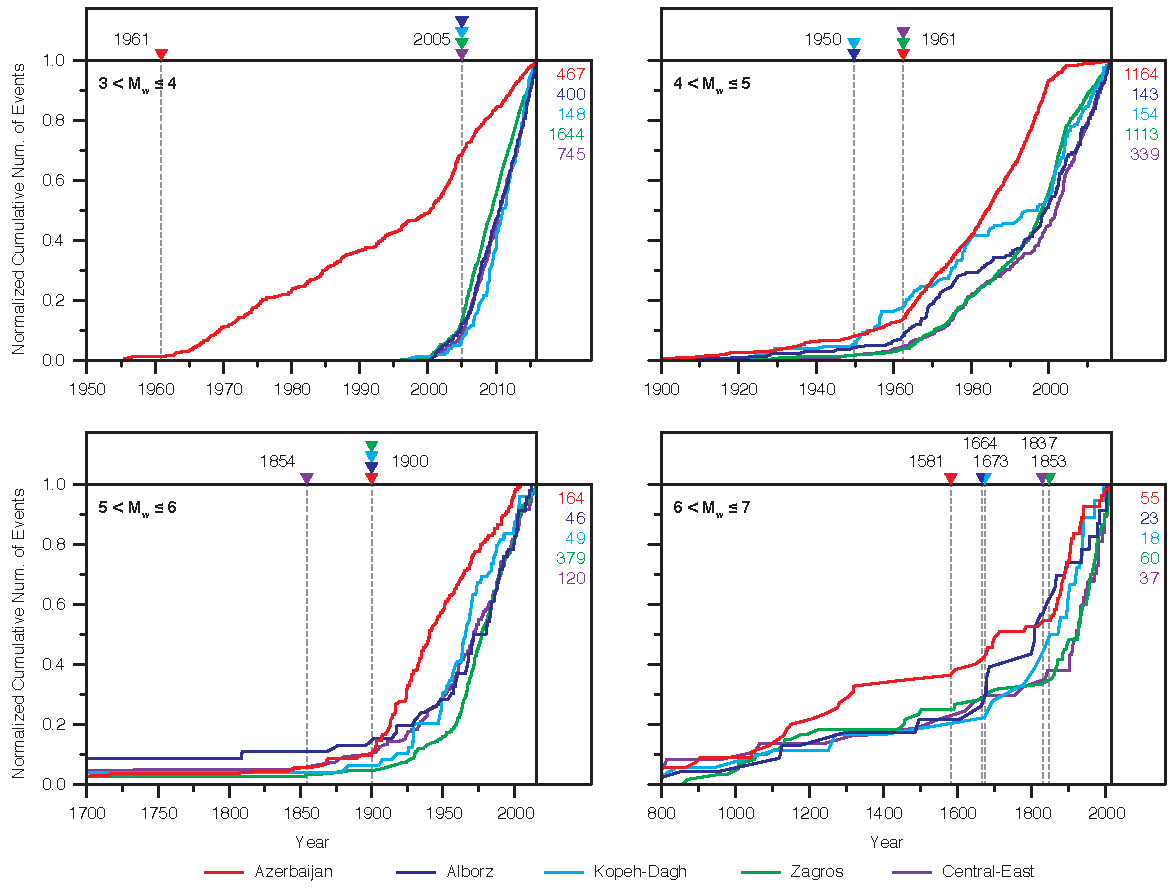
\includegraphics[width=0.8\textwidth]{figures/pdf/figure-05.pdf} 
    \caption{Normalized cumulative number of events and completeness year thresholds for each of the seismic zones considered within the region of interest, and for magnitude intervals of $\Delta M = 1$ between $M_w$ 3 and 6. The year thresholds are indicated by a triangle mark at the top and the vertical dashed lines in the background. Normalization values for each curve are indicated on the right margins and distinguished by color as indicated in the legend.}
    \label{fig:completeness}
\end{figure*}

\subsection{Completeness}

An important aspect of seismic catalogs is their completeness. This characteristic is measured in terms of the start-year of completeness and the completeness magnitude, which are both parameters that are later used in the seismic analysis process. The start-year of completeness is the point in time at which catalog data exhibit a steady rate of event occurrence or record accumulation for a certain magnitude range, and the completeness magnitude ($M_c$) is the magnitude above which the seismic catalog of a region can be considered complete within a certain time period.

The start-year of completeness is commonly identified by inspection. A simple approach used by \citet{Frankel1995} and others is to select the year at which a plot of the cumulative number of events with respect to time becomes (or starts to resemble) a straight line. This is done for different magnitude ranges. Following this approach, we determined the year of completeness for magnitude ranges 3--4, 4--5, 5--6 and 6--7. Our choices are illustrated in Fig.~\ref{fig:completeness}, where we show the normalized cumulative number of events with time for each of the seismic zones and magnitude ranges, and indicate our selection of the year of completeness in each case. The values shown in this figure and those corresponding to the uniform model of the entire region of interest are summarized in Table \ref{tab:completeness}. For events $M_w>7$, in which case there are insufficient data to determine a proper threshold, we assumed the catalog to be complete from the earliest time at which there is record of large magnitude earthquakes. 

Determining the completeness magnitude $M_c$, on the other hand, is often determined using simple numerical analysis in combination with data inspection. Two common approaches are maximum curvature and the goodness-of-fit test methods. The maximum curvature method, or MAXC for simplicity, is widely used because as it has been implemented in the ZMAP software package for seismic hazard analysis developed by \citet{Wiemer2001}. \citet{Zare2014}, for instance, used this software to identify $M_c$ values for the different regions of the Middle East. We use the goodness-of-fit test method introduced by \citet{Wiemer2000}, and compute $M_c$ for different catalog-time intervals, namely 1800--1899, 1900--1999, 2000--2015, and for the complete regional catalogs.

We defined these year intervals based on the data magnitude-time distribution (see Fig.~\ref{fig:scatter}) and the idea of distinguishing between historical, early-instrumental, and modern-instrumental catalogs. Having augmented the original catalog with $M>3$ earthquakes beginning in 2000 also influenced our choice of the intervals because at this point the uniformity of the catalog is altered. Last, we also computed $M_c$ values for the complete regional catalogs, but in this case, in order to maintain uniformity throughout time, we only considered $M>4$ events. Fig.~\ref{fig:mc} illustrates the selection of $M_c$ for the case of the main three northern Iran seismic regions, and Table \ref{tab:completeness} presents the final selection of $M_c$ values for these and the other regions, including the uniform northern Iran model for the complete region of interest.

The values of $M_c$ for different time intervals and seismic regions are used to determine the seismicity Gutenberg-Richter parameters $b$ and $M_{\max}$ (see Section \ref{sec:params}), and the $M_c$ values for the complete regional catalogs and the start-years of completeness are used later for computing the hazard. Admittedly, the choice of the start-years is highly subjective. We should note then, that in the process of choosing the points indicated in the plots shown in Fig.~\ref{fig:completeness}, we considered additional contributing information such as the history of instrumentation. It is well known that the number of recorded earthquakes increased considerably after the first deployment of seismic instruments in the early 1900s, and later with the establishment of the Worldwide Standardized Seismograph Network in 1961. We compared our choices with the year thresholds reported by \citet{Zare2014}, which we found to be consistently earlier than our preferred years of completeness. In the end, our selection should lead to a slightly more conservative estimations of hazard. For the case of $M_c$, we compared our results with the values reported by \citet{Karimiparidari2013} and \citet{Khodaverdian_2016_BSSA} and found them to be in general good agreement, despite differences in the spatial definition of the seismic zones.

\begin{figure*}[t]
    \centering
    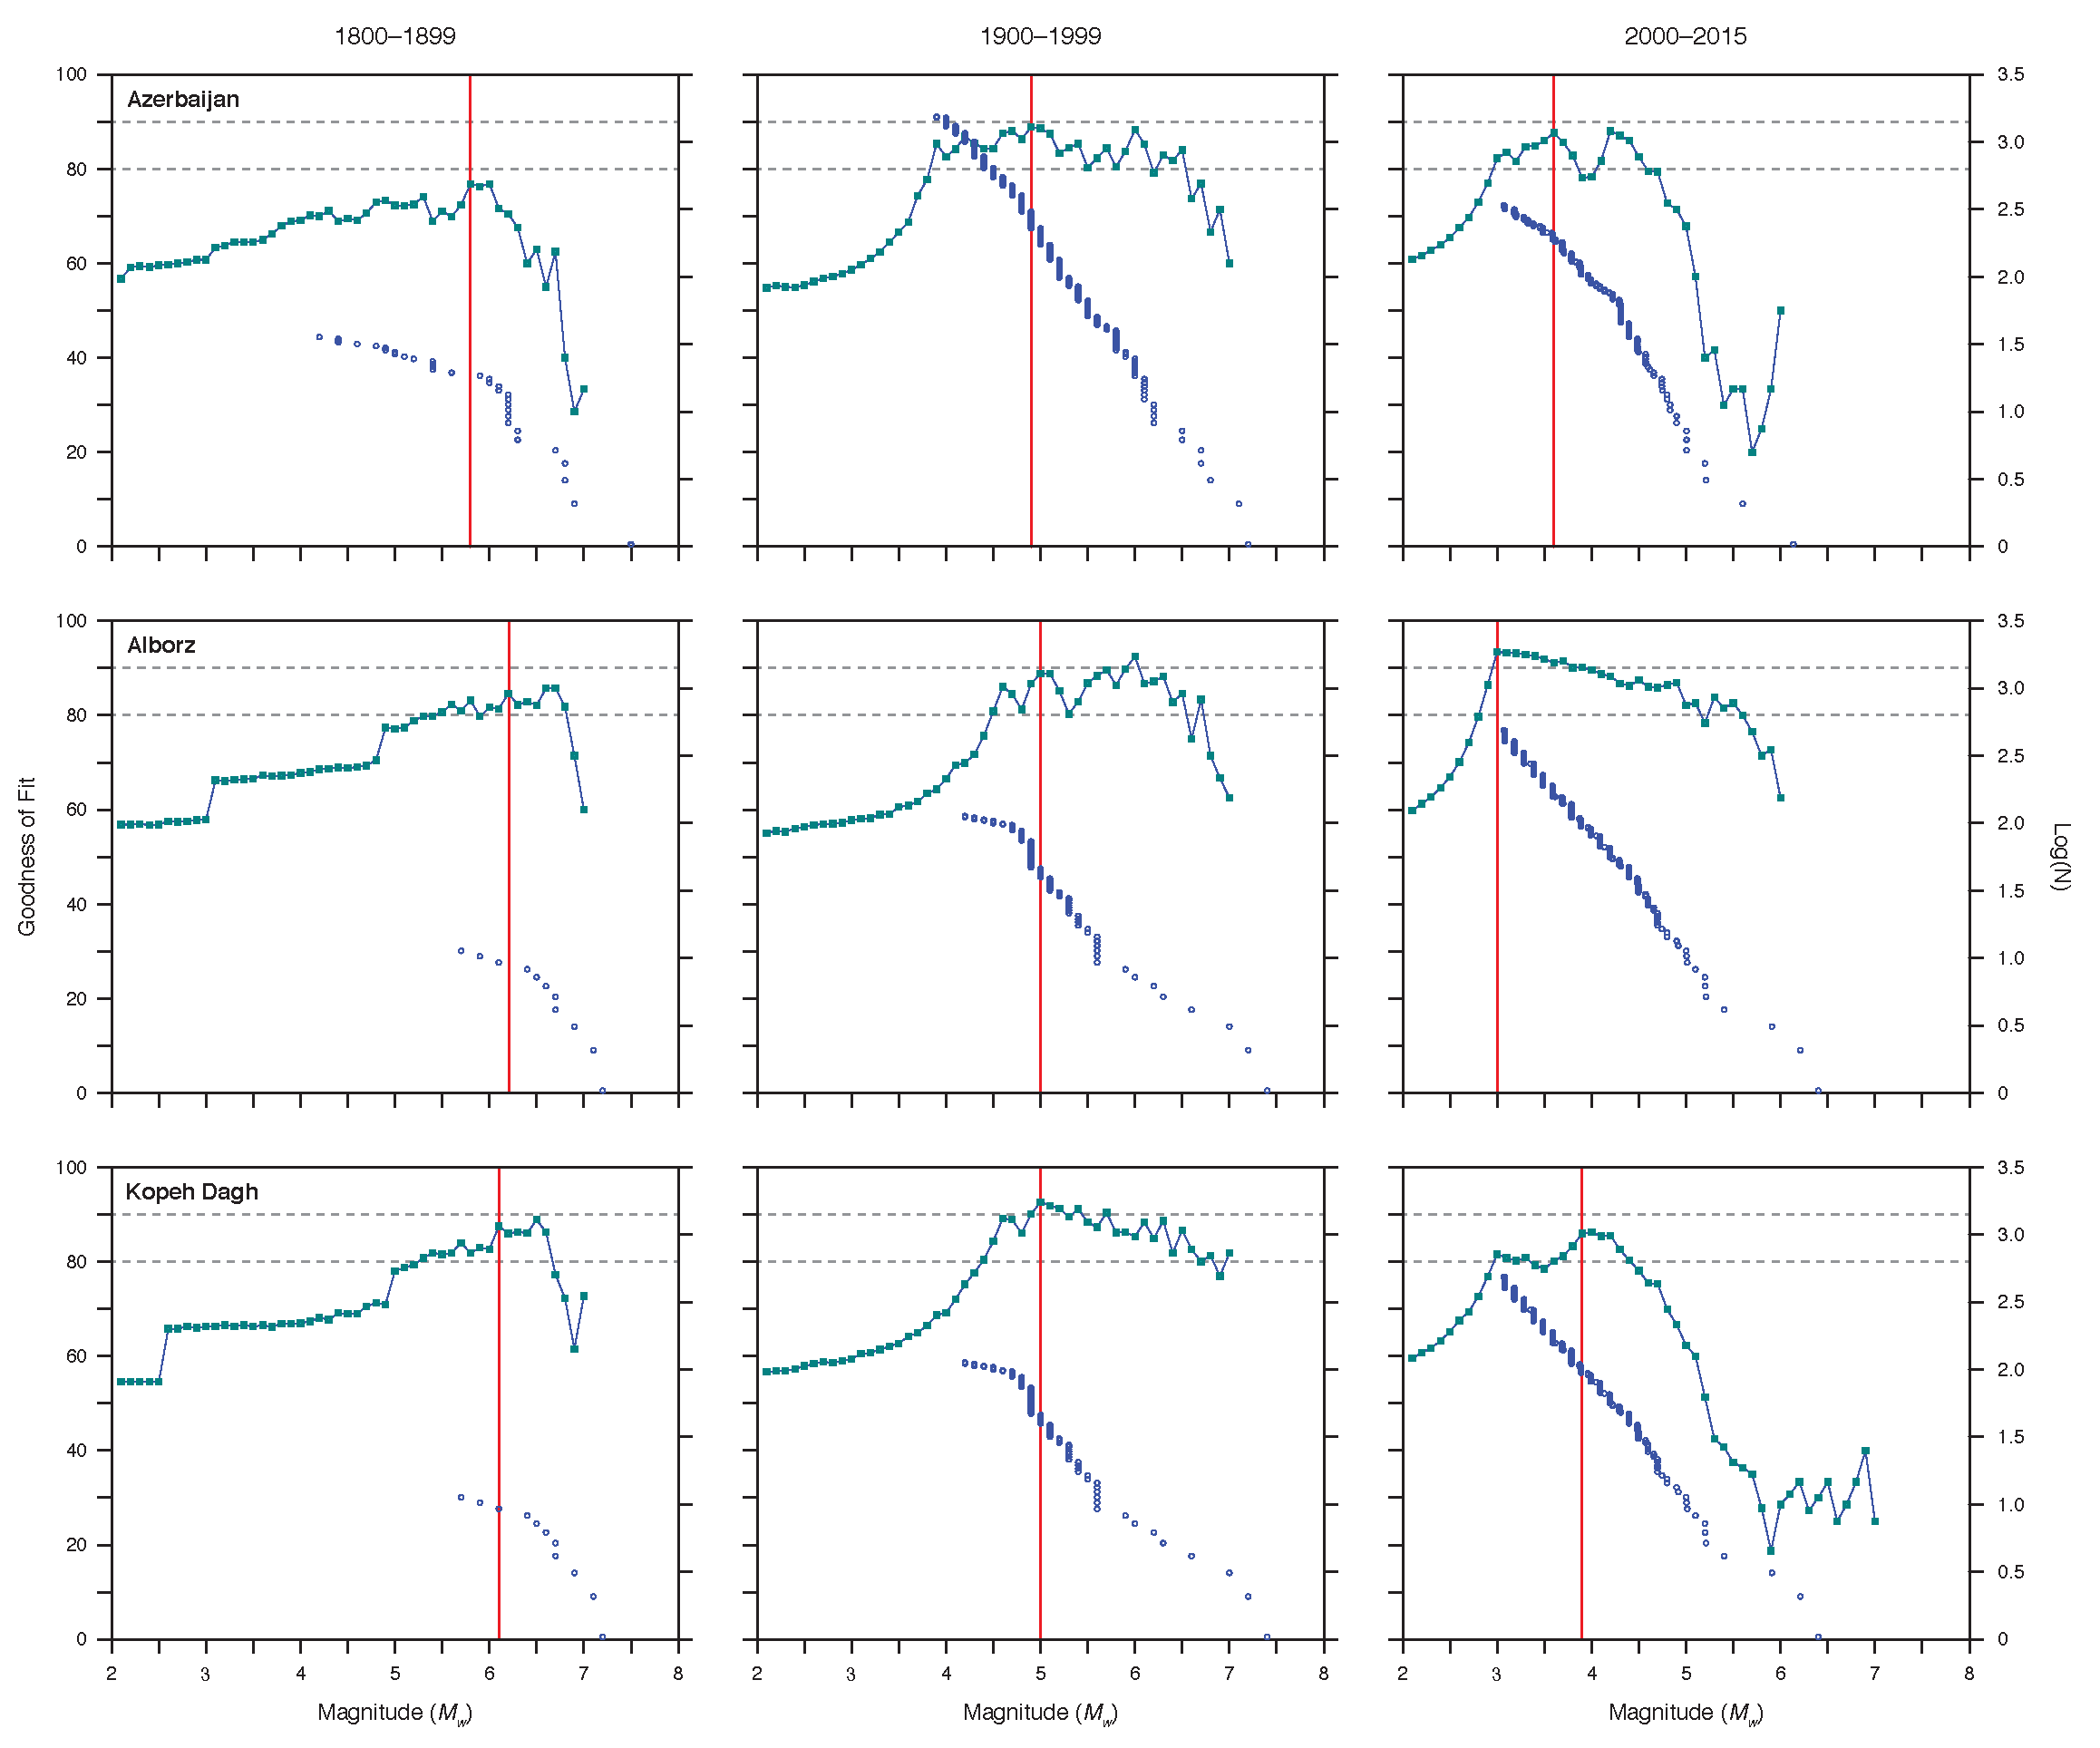
\includegraphics[width=\textwidth]{figures/pdf/figure-06.pdf} 
    \caption{Selection of completeness magnitude ($M_c$) values for the three main seismic regions in northern Iran. The blue squares indicate the computed goodness-of-fit test values and the green circles indicate the cumulative number of events. Both are shown as functions of the earthquake magnitude. The former is plotted in linear scale (left axes) and the latter is plotted in logarithmic scale (right axes). The horizontal dashed lines indicate desired thresholds for the goodness-of-fit values at 80 and 90 percent. The vertical red lines indicate the chosen $M_c$ values for each zone and catalog year interval.}
    \label{fig:mc}
\end{figure*}

\begin{table*}%[t]
    \centering
    \caption{Year thresholds and magnitude completeness for the seismic zones within the region of interest in this study. Year of completeness is provided for magnitude ranges between 3 and 7, with $\mathrm{\Delta}M = 1$. The completeness magnitude is provided for the sub-catalogs for three year intervals.}
    \begin{tabular}{lccccrcccccc}
        \cline{2-12}                                                                                  			\\[-1.6ex]
                        & \multicolumn{5}{c}{Year for $M_w$ ranges} 
                                                            & & \multicolumn{3}{c}{$M_c$ for sub-catalogs} & &$M_c$\\
        \cline{2-6} \cline{8-10}                                                                      			\\[-1.6ex]
                        & 3--4 & 4--5 & 5--6 & 6--7 & \multicolumn{1}{c}{$>7$} 
                                                            & & 1800--1899 & 1900--1999 & 2000--2015  & & Whole	\\[0.6ex]
        \hline                                                                                        			\\[-1.6ex]
        Azerbaijan      & 1961 & 1961 & 1900 & 1581 & 1042  & &     6.0    &     5.0    &     4.2     & &  4.2 	\\
        Alborz          & 2005 & 1961 & 1900 & 1664 &--401  & &     6.2    &     5.0    &     3.5     & &  4.3 	\\
        Kopeh Dagh      & 2005 & 1950 & 1924 & 1673 &    9  & &     6.1    &     5.0    &     4.0     & &  4.9 	\\
        Zagros          & 2005 & 1961 & 1950 & 1853 & 1439  & &     5.3    &     4.8    &     3.9     & &  4.8 	\\
        Central-East    & 2005 & 1961 & 1900 & 1837 &  762  & &     5.5    &     4.8    &     4.0     & &  4.8 	\\
        Uniform Model   & 2005 & 1961 & 1900 & 1778 &--401  & &     6.1    &     4.8    &     3.8     & &  4.8 	\\[0.5ex]
        \hline 
    \end{tabular}
    \label{tab:completeness} 
\end{table*}








% *********************************************************************************************************************
% *********************************************************************************************************************

% ***** In addition, \citet{Zare2014} provided the catalog completeness for different magnitude ranges using the cumulative frequency-magnitude distribution of \citet{Gutenberg1944} and \citet{richter1958}, and the frequency magnitude distribution obtained using ZMAP \citep{Wiemer2001}, and found these methods to yield consistent results. 

% **** Our analysis of this dataset indicated that the catalog satisfies completeness from 2005 onward. 

% *********************************************************************************************************************
% *********************************************************************************************************************

% \citet{Zare2014} uses both historical data prior to 1900 and instrumental data up until 2006, including events from Afghanistan, Pakis\-tan, Saudi Arabia, the Caucasus and parts of Turkey, in addition to the Alborz-Azerbaijan, Zagros, central Iran, Kopeh-Dagh and Makran seismic zones. 

% All events in this catalog are converted to $M_w$ using relationships derived by the authors and by \citet{Escordilis_2006_JS}; and declustered using various methods \citep{Gardner1974, Reasenberg1985, Uhrhammer_1986_EN}. 

% This catalog is particularly relevant because it is published as part of the current effort by the Global Earthquake Model (GEM) partnership and the Earthquake Model of the Middle East (EMME) project.

% In this study we adopt the catalog compiled by \citet{Zare2014} for both historical and instrumental earthquakes. This catalog includes events of magnitude $M_w \geq 4$ from 550 A.d.~to December 1999. 

% We complemented it with events $M \geq 3$ occurred between January 2000 and December 2015 obtained from the IIEES database. 

% The result of our compilation is shown in Fig.~\ref{fig:catalog}, which includes maps for historical and instrumental seismicity. 
% The following sections provide additional details about magnitude conversion and de\-clustering of the events in our combined catalog.

% The portion of the catalog obtained from IIEES for $M \geq 3$ earthquakes between 2000 and 2015 contained event reports that use different magnitude scales. We converted all events with magnitudes in $M_L$, $M_s$, and $mb$ scales to $M_w$ using the same conversion relationships used by \citet{Zare2014}, which allowed us to preserve compatibility with the historical and instrumental seismicity catalog adopted from the same work of \citet{Zare2014}. 

% Last but not least important, we declustered the catalog prior to using it in the assessment of seismic hazard for the region of interest. This entailed the removal of foreshocks and aftershocks from the catalog to adjust the dataset to include only those events in agreement with a Poissonian model, which is a well-accepted model for seismic sources. Out of the original 7,478 earthquakes in the assembled catalog for the seismic regions of Azerbaijan, Alborz and Kopeh-Dagh, we removed 605 foreshocks and 2,917 aftershocks. The resulting final set of events in the catalog compiled for this study is shown in Fig.~\ref{fig:catalog}, which includes maps for both historical and instrumental seismicity.

% *********************************************************************************************************************
% *********************************************************************************************************************

% Naeem's original Text
% ---------------------

% \subsection{Historical  and Instrumental Seismicity}

% Uniform earthquake catalog is the most important factor in seismic hazard analysis of a region.  Different studies have been conducted in order to prepare a uniform catalog for Iranian Earthquake. Historical event interpretation and different magnitude conversion relationships are some of the factors which make all these catalogs different. Among different sources \citet{Ambraseys2005}, \citet{Berberian1994}, and \citet{moinfar1994} are some of the main sources for Iranian earthquake catalog. These catalogs contain historical and instrumental earthquakes that have been reported in literature and national and international networks. According to \citet{Ambraseys2005}, there are some scattered indication of earthquake effects  back to third millinuim BC. However, adequate documentary coverage of individual events begins from seventh century A.D. \citet{Mirzaei1997} provided a comprehensive list of studies that have been done in compilation a uniform catalog for Iranian earthquakes in order to prepare a uniform catalog of earthquake (all earthquakes are converted to surface wave magnitude Ms) for seismic hazard assessment in Iran. The catalog is covering the period of 4th century B.C. through 1994. The instrumental data is achievable from three national agencies including IIEES, International Institute of Earthquake Engineering and Seismology; IRSC, The Iranian seismological center, University of Tehran; and BHRC, Building and Housing Research Center (Iran Strong Motion Network) (For more information about these networks see \citet{Karimiparidari2013}).

% Many most of attenuation relationship use  moment magnitude $M_w$ as an input for the equation \citep{Douglas2011}. Moment magnitude is not suffering from saturation and has physical meaning \citep{Kanamori1977}. Due to mentioned reasons Mw has become a most appropriate magnitude scale in recent studies. 

%  \citet{Karimiparidari2013}compiled a uniform earthquake catalog for Iran and adjacent areas, using international and national databanks until April 2010.  They developed relationships between moment magnitude and other magnitude based on orthogonal regression.  They removed the dependent events (aftershocks and foreshocks) using the procedure by \citet{Gardner1974}. The catalog of events with magnitude equal and above Mw 5.5 is provided. 
% \citet{Shahvar2013} presented a unified and homogeneous catalog for the Iranian plateau $(M_w >= 4)$, created by merging data from two local catalogs and seven international agencies for 1900-2011 period. They used orthogonal regression method \citep{Castellaro2006} to derive magnitude conversion relation. By removing foreshocks and aftershocks according to the procedure detailed in Uhrhammer(1986), they also provided declustered version of the catalog.

% The recent unified catalog for Middle East region is published as a part of Global Earth Model (GEM) and the Earthquake Model of the Middle East (EMME) project by \citet{Zare2014}. They used all historical (pre-1900), early and modern instrumental events up to 2006. The catalog contains data from Alborz-Azerbaijan, Afghanistan-Pakistan, Saudi Arabia, Caucasus, Central Iran, Kopeh-Dagh, Makran, Zagros, and part of Turkey. The magnitude of all events are converted to Mw through relationships which is derived at previous studies or newly derived at the study relationships. They declustered data through different methods including \citet{Gardner1974}, Uhrhammer(1986), \citet{Reasenberg1985}, and Gruenthal. \citet{Zare2014} provided the catalog completeness for different magnitude range using  the cumulative frequency-magnitude distribution of  \citet{Gutenberg1944} and \citet{richter1958}, and frequency magnitude distributaion of ZMAP \citep{Wiemer2001} software. The methods confirms the results of each other. 

% In this study we consider earthquakes with Mw equal and greater than 3. Earthquakes with magnitude 3 are not considered as a structural threat, however, the epicenter of earthquakes with magnitude $M_w 3$ are a  susceptible location for future bigger earthquakes.  According to our preliminary data processing based on IIEES data, Iranian catalog for earthquake with magnitude greater and equal 3, is complete from 2005. In order to make sure about the completeness of the catalog, we use IIEES data from 2000. We used the EMME project data provided by \citet{Zare2014} up to 2000. Fig.~\ref{fig:historical} represents the historical data (pre 1900) in the study region. 

% \subsubsection{Magnitude Conversion}

% The catalog of recorded earthquake from 2000-2015 which is downloaded from IIEES is reported the earthquake based on different magnitude scale. We converted the $M_L$, $M_s$, and $mb$ magnitudes through conversion relationships which is defined in \citet{Zare2014}. There also some of data which is recorded in $M_D$ (Duration magnitude). These data are reported by International Seismological Centre (ISC).  \citet{Deniz2010}, developed a set of empirical equations to convert earthquake magnitudes in $mb$, $M_D$, $M_L$ and $M_s$ scales to the $M_w$ scales using orthogonal regression procedure. They used data of earthquake that occurred in Turkey from different data centers including ISC. In this study we use the conversion equation of \citet{Deniz2010} to convert the Md to Mw. Although they defined the equation based on $M_w>=4.5$, we extrapolate the equation for lower magnitude. We believe having those earthquakes, even with small error  in magnitude is important for estimating an accurate "a" value  in Gutenberge-Richter equation.

% \begin{figure*}[!ht] 

% \centering
% \includegraphics[scale=0.4]{figures/pdf/Figure2.pdf} 
% \caption{Historical earthquakes of Iran (pre 1900). Different colors represent different year of occurrences and size of circles are proportional to the earthquake magnitude. }
% \label{fig:historical}
% \end{figure*}

% \subsubsection{Declustering}

% It is generally assumed that the seismicity of each tectonic seismic source follows a Poissonian occurrence process. Therefore, in order to accomplish this, we declustered the earthquake catalog. In compiling the catalog of events, foreshocks and aftershocks were removed using a declustering methodology \citep{Gardner1974}. For north Iran (lon: 42-62.5, lat: 33-41), from 7478 earthquake event we removed 605 Foreshocks and 2917 aftershocks.
% Whole data that we used for seismicity parameters of Zagros and Central Iran tectonic seismic regions are not included in these numbers. Fig.~\ref{fig:instrumental} shows the epicenter of declustered instrumental  earthquakes.

% \begin{figure*}[!ht] 

% \centering
% 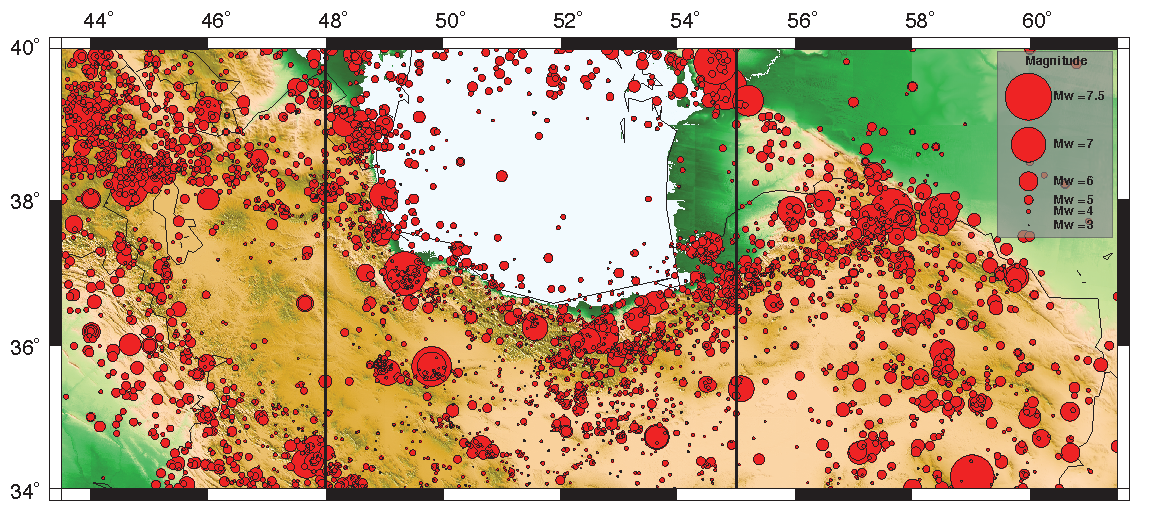
\includegraphics[scale=0.25]{figures/pdf/Figure3.pdf} 
% \caption{Declustered instrumental seismicity map (after 1900) of Northern Iran. The study areas are separated at longitude of 48$^{\circ}$ and 55$^{\circ}$ . } 
% \label{fig:instrumental}
% \end{figure*}

% \subsection{Divisions}

% As we discussed earlier (see the Introduction section), classifying the tectonic seismic regions has been a controversial debate. In this study we consider two seismic tectonic models. First model is according to \citet{Mirzaei1998} and \citet{Karimiparidari2013} classification, which includes Azerbaijan, Alborz, Kopek Dagh, and part of Central Iran, and Zagros, the second model is a uniform model for the whole north Iran.  
